\section{Designing and Implementing Rich \Glspl{exp} with \Glspl{name}}

\shortchange{We designed and implemented \glspl{exp} for 3 languages.
\if 0 As we describe these efforts, we highlight design inspirations and implementation details pertinent to generating helpful explanations.\fi} 
For each, we aim to generate useful explanations for a range of possible code examples without knowing the precise content ahead of time. 
We discuss techniques for natural language explanations, document generation, template instantiation, and common usage mining to construct \glspl{exp} for CSS selectors, regular expressions, and wget.
\if 0 Our techniques show how to automatically generate useful examples, reusing and repurposing existing documentation by reusing its codebase, and, where manual effort is needed, guide that effort to the most useful cases by extracting frequency information from the web. \fi

\subsection{CSS Selectors}

CSS selectors appear in JavaScript, stylesheets, and web scrapers.
Despite their small size, advanced and compound CSS selectors cause errors for programmers working with HTML and CSS~\cite{park_towards_2013}, making them an appropriate language for developing effective automatic \glspl{exp}.

\subsubsection{Explaining CSS Selectors with natural language}

Our method of building natural language explanations for CSS selectors involves language generation through parse tree traversal.
Our English language explanation technique is implemented as a tree walker that starts at a leaf node and climbs up through its ancestors.
The walker first generates a clause at a leaf node that consists of a single noun --- a description of the element's tag type in plain English (e.g., `link' instead of the anchor tag `a', and `bolded text' instead of `strong').
\begin{changes}
It then appends modifiers to the noun to describe the ID, classes, attributes, and pseudo-selectors for the node which must be present for the node to be selected.

Then the walker ascends.
At each ancestor, it forms a phrase that its child selector is picked ``from'' the parent (see Figure~\ref{alg:css_traversal}).
When it reaches the root, the walker completes a sentence describing that the selector shown chooses the child via all of its ancestors.
\end{changes}
English language is realized using SimpleNLG\footnote{\url{https://code.google.com/p/simplenlg/}}.
We show descriptions we generate in Table~\ref{tab:css_descriptions}. 
% \marti{This is a not a complete explanation of how the NLP is done ... how is the Start of the sentence generated, the word "chooses" generated, etc.}

\begin{figure}
\begin{algorithmic}
\scriptsize

\Function{visit\_node}{node}
    \If{node has id}
        clause = node.element
	\State{clause += ` with ID $node.id$'}
    \Else{}
    \State{clause = pluralize(node.element)}
    \If{node has class}
        \State{clause += ` of class $node.class$'}
    \EndIf{}
    \EndIf{}
    \If{node has child}
        \State{child = visit\_node(node.child)}
        \State{clause += child + `from' + clause}
    \EndIf{}
    \State{\Return{clause}}
\EndFunction{}

\end{algorithmic}
\caption{A recursive function for generating an explanation of a CSS selector from a tree of elements and their attributes.}
\label{alg:css_traversal}
\end{figure}

\newcolumntype{S}{>{\scriptsize\arraybackslash}m{6cm}}
\newcolumntype{T}{>{\scriptsize\arraybackslash}m{9cm}}

\begin{table*}[t]
\caption{Text Generated to Explain CSS Selectors}
\label{tab:css_descriptions}
\centering
\begin{tabular}{ST}
\toprule
\headrow{Selector} & \headrow{Realized Text} \\
\midrule
\texttt{div.video-summary-data a[href\^=/video]} & The selector `div.video-summary-data a[href\^=/video]' chooses links with URLs starting with `/video' from containers of class `video-summary-data'. \\ \midrule
\texttt{input:focus} & The selector `input:focus' chooses in-focus inputs. \\ \midrule
\texttt{p.introduction::text} & The selector `p.introduction::text' chooses text from paragraphs of class `introduction'. \\ \bottomrule
\end{tabular}
\end{table*}

\subsubsection{Generating example documents}

% To demonstrate what CSS selectors choose, we build example HTML documents with elements that can be matched by the selector.
\begin{changes}
Selectors refer to node characteristics and parent-child and sibling relationships manifest in HTML\@.
We reverse engineer simple documents for which those characteristics and relationships hold.
\end{changes}
% This structure can be understood by navigating and inspecting the HTML.\@
\if 0
We gain motivation for this \gls{exp} from the knowledge that programmers must understand the structure of the document before writing selectors that leverage that structure, and that this structure is most often represented through HTML\@.
\fi

Our generation technique is implemented as a visitor for the parse tree of a CSS selector.
For each node that represent the tag of an HTML element, we use PyQuery\footnote{\url{https://pypi.python.org/pypi/pyquery}} to construct an HTML element.
The visitor starts at the leaf nodes of the tree.
As it ascends, the visitor constructs the document by appending child nodes to their parent.
The resulting document is pretty-printed with BeautifulSoup\footnote{\url{http://www.crummy.com/software/BeautifulSoup/}} with spaces, newlines, and carets escaped for display in the browser.

\if 0
As an example, consider the \texttt{``table tr td''} selector (Figure~\ref{fig:html_table}).
The parse tree the \Gls{name} produced consists of 3 nodes --- the \texttt{table} at the root, the \texttt{tr} as \texttt{table}'s only child, and \texttt{td} as the only child of \texttt{tr}.
The visitor for the CSS \Gls{name} constructs an HTML node, first visiting the \texttt{td} element to generate node \texttt{<td></td>}.
It next visits the \texttt{tr} node, where it creates node \texttt{<tr></tr>} and appends the \texttt{<td></td>} element as a child.
Finally, it reaches the root node, \texttt{table}, where it constructs a \texttt{<table></table>} node and appends \texttt{<tr></tr>} as the table's child.
\fi

To convey that the leaf nodes are the elements the selector chooses (rather than all elements in the generated document), leaf nodes are marked with a \texttt{span} to bolden and color the element.
If an element has no tag name, we create a generic \texttt{div} to represent it.
Attributes, ids, and class names are added to the opening tag of the element.
As pseudoclasses like \texttt{checked} and \texttt{hover} are not visible from the document but valid components of selectors, we demonstrate their presence as comments within the element that was selected~\ref{fig:html_pseudoclass}.

Future iterations of CSS \glspl{exp} might benefit from rendering the documents as they would appear when viewed in a browser, particularly for graphical elements like tables and form inputs.
\if 0
Example documents that we automatically generate for real code we found in online programming help are shown in Figure~\ref{fig:selector_demonstrations}.
\fi
\if 0
\bjoern{After the submission deadline, let's revisit this technique --- I think there is a much larger design space here of showing other candidate trees that match, as well as trees that do not match. Also, we may want to indicate that selectors return collections by repeating elements --- e.g.\ td  siblings, or two different tables in the same document.}
\andrew{Roger.  Yes, I think there's a lot to do with this case of example generation.}
\fi

\begin{figure}
\centering{%
    \subfiguretopcaptrue{}
    \subfigure[\tiny{\texttt{form.myform}}]{%
        \raisebox{-0mm}{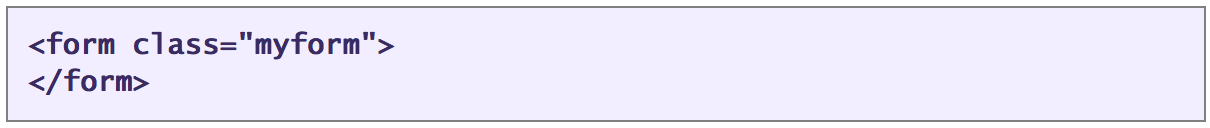
\includegraphics[width=.3\columnwidth]{figures/html_form_myform}\label{fig:html_form.myform}}
    }
    \subfigure[\tiny{\texttt{table tr td}}]{%
        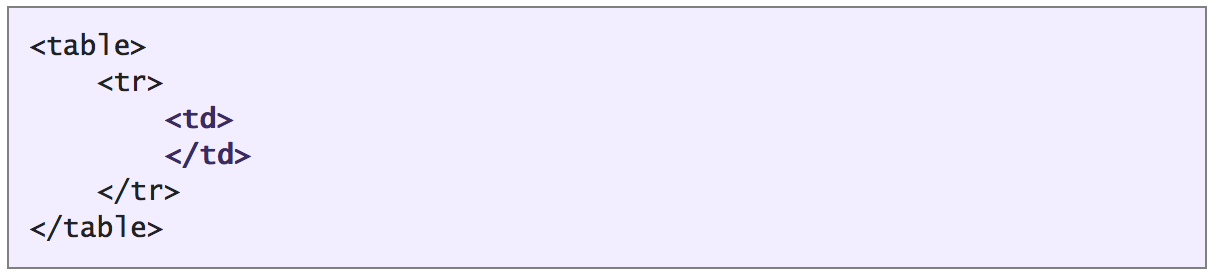
\includegraphics[width=.18\columnwidth]{figures/html_table}\label{fig:html_table}
    }
    \subfigure[\tiny{\texttt{\#first:hidden}}]{%
        \raisebox{-0mm}{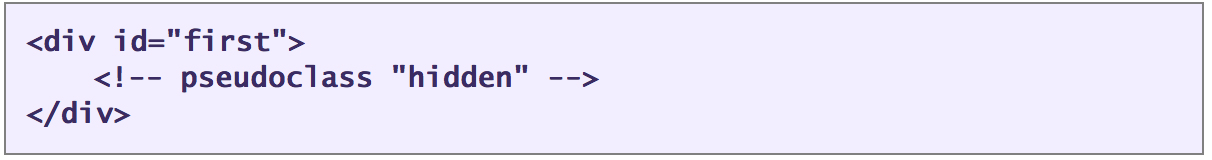
\includegraphics[width=.4\columnwidth]{figures/html_pseudoclass}\label{fig:html_pseudoclass}}
    }
    \caption{Examples of HTML documents that can be matched by a CSS selector, automatically generated by our CSS \Gls{name}.
    Note that we bolden the font of the selected node, for example in subplot~\ref{fig:html_table}, where the selected element in the \texttt{td} nested inside a \texttt{tr} in a \texttt{table}.}\label{fig:selector_demonstrations}
}
\end{figure}

\subsection{Regular Expressions}

\begin{changes}
Regular expressions can be difficult for novices and time-consuming for experts to understand.
There is a plethora of tools to automatically that generate token-by-token explanations of patterns\footnote{\url{http://rick.measham.id.au/paste/explain.pl}}, visualize them\footnote{\url{http://regexper.com/}}, and help programmers debug them\footnote{\url{https://www.debuggex.com/}}.
We discuss techniques for visualizing and explaining regular expression by reappropriating third-party tools generating example strings.
\end{changes}

\subsubsection{Explaining Expressions through Diagrams via 3rd-Party Visualizations}

In an early prototype, we developed a  \Gls{name} for visualizing regular expressions, leveraging the 3rd-party regular expression visualizer called \emph{RegExper} (Figure~\ref{fig:regex_visualization}).
While the technical implementation details are trivial, we mention it here as an example that a \Gls{name} author can leverage demonstrations produced by their peers to create \glspl{exp}.

\begin{figure}
\centering
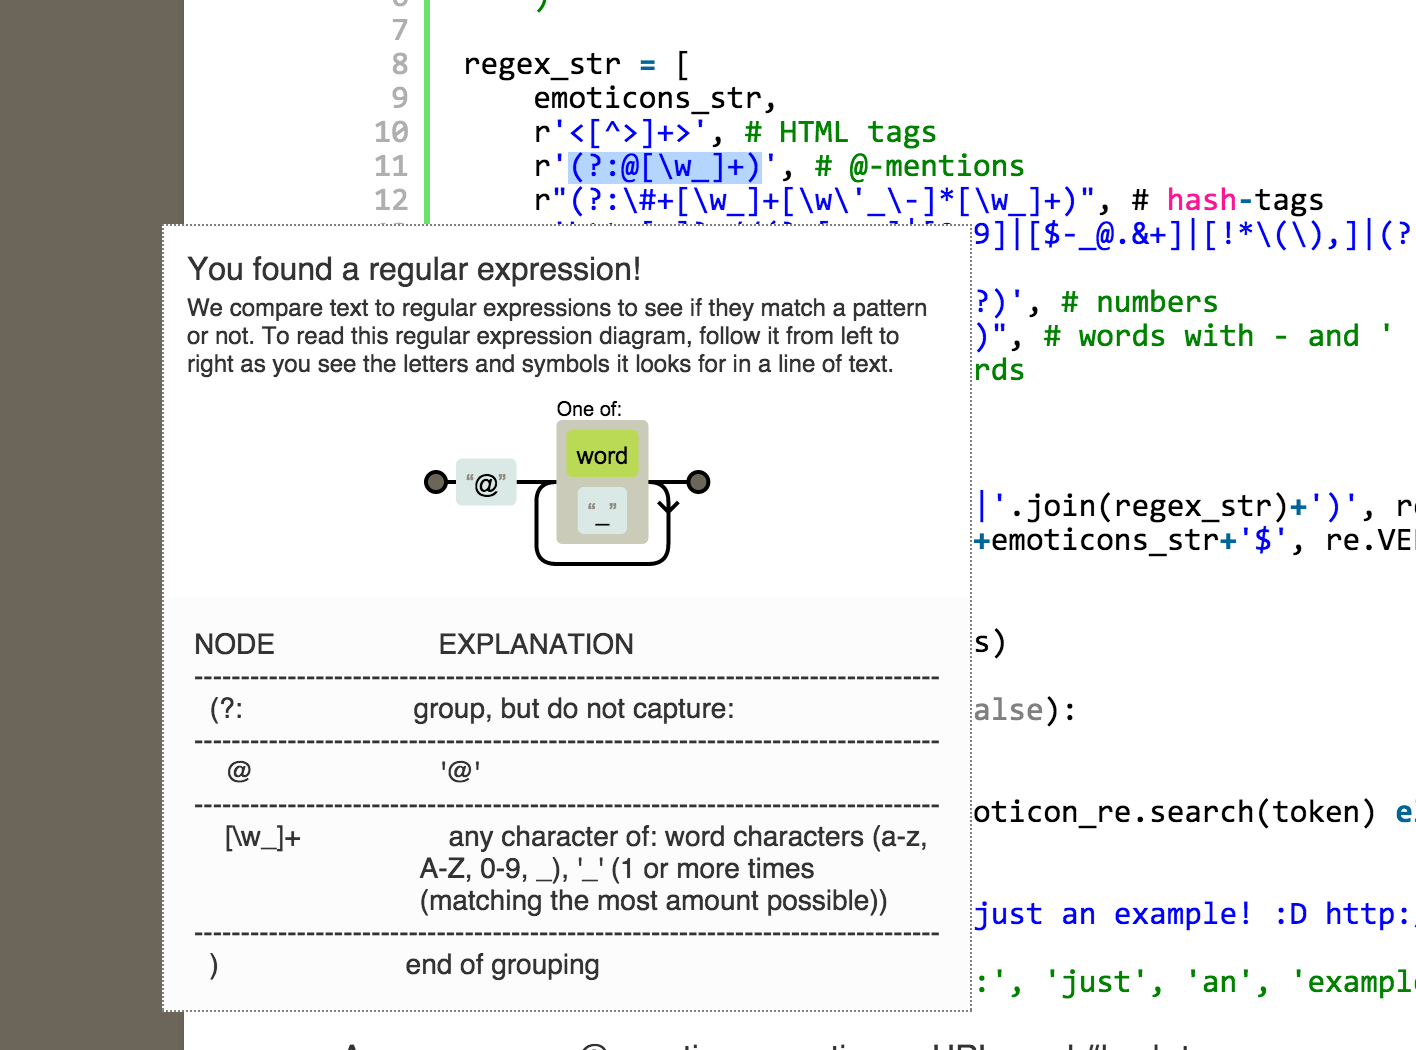
\includegraphics[width=\columnwidth]{figures/explain_on_select}
\caption{A \gls{exp} of a regular expression that adapts content from the third-party tools \emph{Regexper} and \emph{explain.pl} into an in-situ tooltip.}
\label{fig:regex_visualization}
\end{figure}

\subsubsection{Generating example expressions}

Inspired by recent work on building counterexample-guided feedback on automaton design problems~\cite{dantoni_how_2015}, we aimed to generate helpful and instructive examples of what a regular expression can match.
The explanation stage we have developed shares thematic ties with the CSS selector document generator. 
\if 0
\bjoern{Do we not have a detector because of a lack of time or because of conceptual roadblocks? Can you find all string literals in a code block, compile a regular expression for it (re.match()) and test whether that produces an error?}
\andrew{Lack of time. Sure --- I can make something that performs this.  Let me get to the preliminary study first and then move onto this.}
\fi

Like the demonstrations for CSS selectors, we choose to generate brief but demonstrative examples, assuming that strings cannot be too long, or else readers will not be able to grasp the core intent of the pattern.
Given a regular expression, we build a parse tree that consists of branches, repetitions and literals by examining output from Python's built-in regular expression compiler.
We generate each sub-pattern marked with a repetition \texttt{*} or \texttt{+} exactly once to ensure the subpattern is represented in the text without adding too much length to the string.
All literals are printed exactly as they appear in the pattern, and we choose a random side of each branch. 

We take effort to produce readable strings.
When we find a repetition of alphanumeric characters, we print an English dictionary word 4-6 letters in length.
If the character class contains symbols or numbers, we insert 2 random non-alphabetic characters from the class.
\if 0
In this way, we insert meaningful sub-patterns based on recognizable words as the constituents from which matching strings are built.
\fi

\begin{figure}
\centering
\setlength{\fboxsep}{10pt}
\noindent\framebox[\columnwidth][c]{%
\begin{minipage}{.95\columnwidth}
\footnotesize{\texttt{([0-9A-F]\{2\}[:])\{5\}([0-9A-F]\{2\})}:} 
\emph{D8:E6:0C:ED:0E:79}
\vspace{.5em} \\
\footnotesize{\texttt{\^{}(\textbackslash{}d\{3\})-(\textbackslash{}d\{3\})-(\textbackslash{}d\{4\})\$}}: 
\emph{307-039-2703}
\end{minipage}
}
\caption{Examples of regular expressions followed by automatically generated example strings.}
\label{fig:regex_strings}
\end{figure}

\subsection{wget}

\begin{changes}
As Miller et al.~\cite{miller_inky_2008} point out, command lines offer efficiency at the price of learning command names and options through an up-front investment of effort.
We created a \Gls{name} for the file retrieval Unix command ``wget'' to show how \Glspl{name} can reduce the effort of recalling the meaning of single-character argument symbols and positional arguments for Unix commands in general.
\end{changes}
wget has around 100 arguments, making it impractical to remember what each individual one means, particularly with its opaque short flags.
Utilities like wget already have comprehensive (albeit non-adaptive) documentation accessible through \texttt{man} pages and the \texttt{-h} flag from the command line that can be used as a starting point for building in-situ documentation.

\subsubsection{Listing command options and extracting help text from source code}

We generate argument-level help extracting and modifying help phrases for each argument as it is written into the wget C code.
Two patterns in original help messages allowed us to build more context-relevant descriptions of the arguments.
(a) Some help messages began with a noun that described what the value represented, e.g., ``location for temporary files created by the WARC writer.''
If we detected that a help phrase started with a noun using a standard typed dependency parser\footnote{\url{http://nlp.stanford.edu/software/lex-parser.shtml}}, we could add the value to the start of the statement, (``\emph{my\_dir is a} location for temporary files created by the WARC writer'').
(b) If the variable name was used in all capital letters in the help (STRING in ``insert STRING into the warcinfo record.''), we just substituted the value of the argument into the help phrase.

\subsubsection{Compound explanations of frequent option groups}

For wget, the intent of a command can be inferred from a combination of options.
For examples, when \texttt{--user} and \texttt{--password} are used together, the caller is authenticating to access a restricted resource.
By using \texttt{-A}, \texttt{-r}, and \texttt{-l} together, programmers recursively scrape a site for files of a certain type, to a depth of following links.

Based on a pilot effort with wget, we propose a way to find common use cases of commands with many options by mining programming help.
We scraped 1000 questions from StackOverflow matching the query `wget'.
From these, we extracted 510 lines of code that began with the string `wget'.
Using a custom wget parser from an earlier version of the wget \Gls{name}, we parsed 346 of these lines without error.
For all lines, we then computed the co-occurrence of options, counting how often certain options were used together.

\if 0
\begin{table}
\caption{Arguments that frequently co-occur in a sample of 500 StackOverflow posts on wget.}
\label{tab:wget_arguments}
\centering
\begin{tabular}{llc}
\toprule
\headrow{Option 1} & \headrow{Option 2} & \headrow{Count} \\
\midrule
\texttt{-r} & \texttt{-A} & 28 \\ \midrule
\texttt{--user} & \texttt{--password} & 23 \\ \midrule
\texttt{-r} & \texttt{-l} & 22 \\ \midrule
%-p & -k & 17 \\ \hline
%-r & -e & 14 \\ \hline
%-r & -P & 13 \\ \hline
%-r & -nd & 12 \\ \hline
\dots & \dots & \dots \\ \bottomrule
\end{tabular}
\end{table}
\fi

\begin{changes}
Commonly co-occurring option pairs include \texttt{-r} and \texttt{-A} (28 counts), \texttt{--user} and \texttt{--password} (23 counts), and \texttt{-r} and \texttt{-l} (22 counts).
These pairs are indeed semantically meaningful:
\texttt{-r}, \texttt{-l}, and \texttt{-A} can be used together to recursively scrape for a certain file type from a site;
and \texttt{--user} and \texttt{--password} are used concurently to authenticate.
\end{changes}

The combination of the \texttt{-r}, \texttt{-l<level>}, \texttt{-A<ext>}, and \texttt{-e robots=off} tags suggest that a user is about to scrape a destination URL recursively to depth level \texttt{l} for files of type \texttt{A}, while disregarding the recommended etiquette for notifying the server that your crawler is a `bot'.
In our wget \Gls{name}, we create compound explanations, or string templates for describing the intent of  these most-frequent groups of options, into which the values of the parameters can be substituted (Table~\ref{tab:wget_combos}).
To reduce the verbosity of text descriptions, we require that any one option can be described in at most one compound explanation.
With the techniques described above, we generated explanations for wget commands like those shown in Figure~\ref{fig:wget_accelerators}.
%
\newcolumntype{L}{>{\scriptsize\arraybackslash}m{5cm}}
\newcolumntype{C}{>{\scriptsize\arraybackslash}m{5cm}}
\newcolumntype{R}{>{\scriptsize\arraybackslash}m{6cm}}
%
\begin{table*}[t]
\caption{Templates for Describing Combinations of wget options}
\label{tab:wget_combos}
\centering
\begin{tabular}{LCR}
\toprule
\headrow{Template} & \headrow{Command} & \headrow{Realized Text} \\
\midrule
Recursively scrape web pages linked from \{url\} of type `\{accept\}', following links \{level\} times. &
\texttt{wget -l3 -A `*.jpg' \urltarget{}} & 
Recursively scrape web pages linked from http://\urltarget{} of type `*.jpg', following links 3 times. \\
\midrule
Authenticate at {url} with username `{user}' and password `{password}'. &
\hangpara{.25in}{1}{\texttt{wget --user andrew --password mypass \urltarget{}}} & 
Authenticate at http://\urltarget{} with username `andrew' and password `mypass'. \\
\bottomrule
\end{tabular}
\end{table*}
%
\begin{figure}
\centering{%
\if 0
    \subfigure[A trivial wget command and an automatically-generated explanation of what it does. \bjoern{Error in figure --- commandline says ``fileurl'' but explanation says 
    ``http://fileurl'' --http isn't automatically prepended by wget. Also, you can skip the simple example if you need space.}]{%
        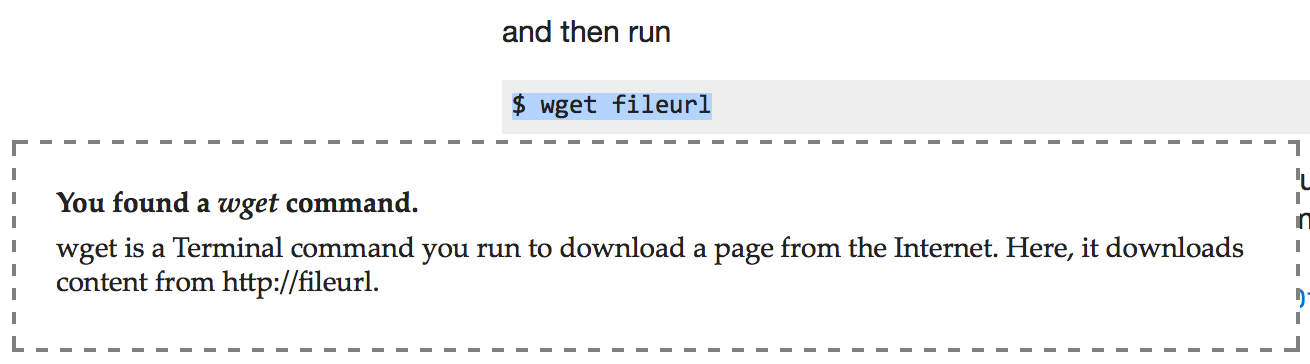
\includegraphics[width=\columnwidth]{figures/wget_trivial}\label{fig:wget_trivial}
    }
\fi
\if 0
    \subfigure[]{\label{fig:wget_complex}}
    \fi
    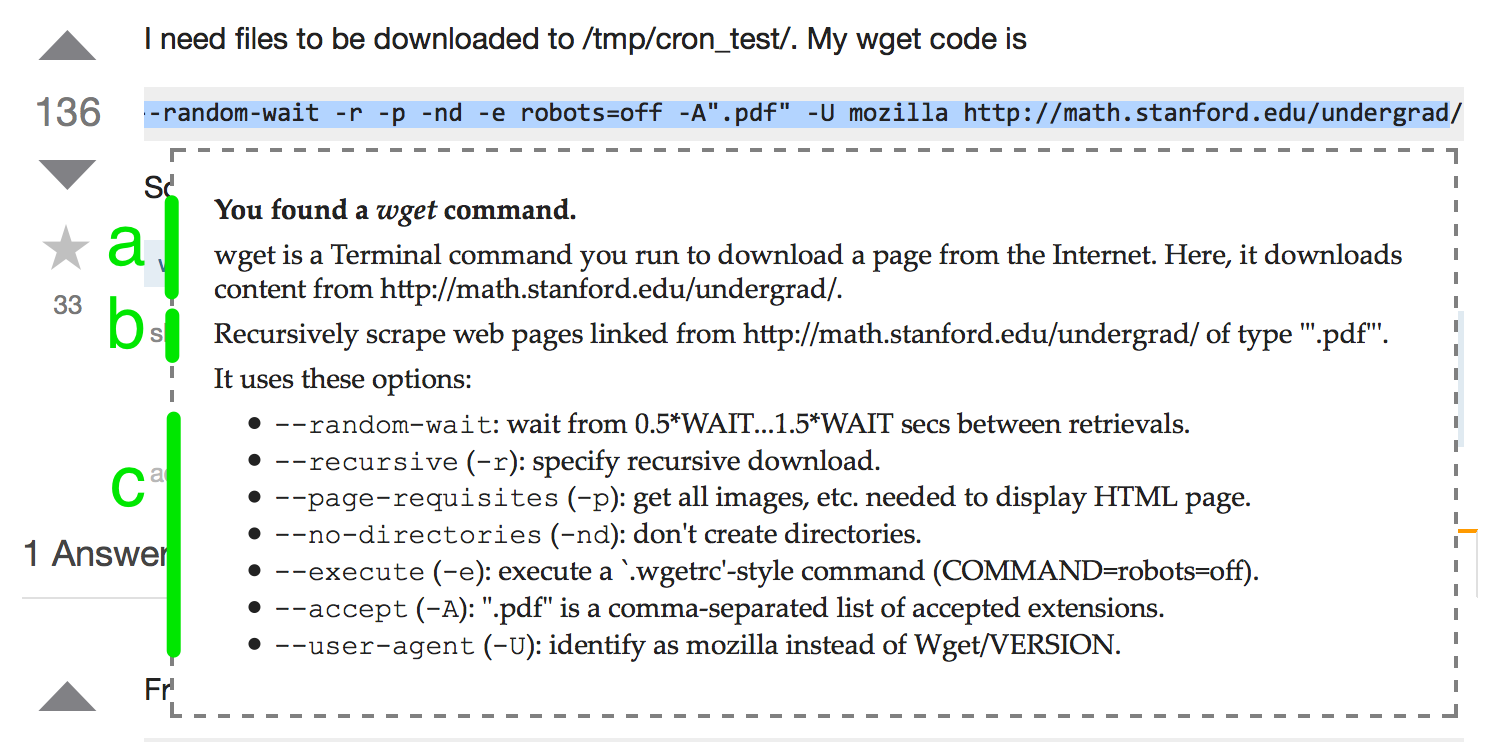
\includegraphics[width=\columnwidth]{figures/wget_complex_explained}
    \caption{%
    A multi-level explanation of wget comprises three parts.
        \emph{(a)} An introduction to the command.
        \emph{(b)} A meaningful description of what this combination of options does at a high level.
        \emph{(c)} A review of the meaning and values of each of the options.
    }\label{fig:wget_accelerators}
}
\end{figure}
%
\begin{changes}
\subsection{Design Guidelines for \Glspl{exp}}
We propose four guidelines to aid in designing \glspl{exp} for languages in online code examples.

First, leverage multiple representations to illuminate high-level intent and low-level understanding of syntax.
We explain CSS selectors and regular expressions with text and examples, and wget with high-level and low-level explanations.
Such a format supports multiple information needs at once, enabling a viewer to grasp the purpose of the code and engage in fine-grained inspection to prepare for modifying it.

Second, be concise --- skip static explanations and focus on dynamically generated content.
Our CSS natural language explanations open with one sentence introducing the purpose of CSS selectors.
Our usability study revealed that parts of explanations that remain unchanged are likely to be ignored. % , implying that conceptual explanations that appear frequently may be overlooked.
% 3 of 9 participants either commented that they were unlikely to read the introductory text because it remained unchanged, or that there was some information they had skimmed over that included an important conceptual point that would have been helpful for them.
% Future \Glspl{name} could keep track of how often and how recently a programmer has seen some explanation.
% Additional studies are needed to determine if template-based explanations dependent on the arguments used are prone to similar skimming or skipping if they do not change sufficiently between very different code examples.

Third, reappropriate existing documentation.
Explanations for the wget \Gls{name} were built from help messages extracted from the utility's source code.
Programmers working with languages like regular expressions have already built visualization and explanation engines used widely within their communities.
The task of the \Gls{name} author, when good tools and documentation exists, is to locate and build mashups of parsers and explainers built by their peers, and then support in-situ explanations by producing a reliable language detector.

Fourth, focus on common usage rather than full grammars.
Common usage can be defined in a data-driven way, rather than relying on intuition.
By parsing CSS selectors from jQuery code on 50 tutorial pages, we found that 233 / 343 (67.9\%) are simple ID or class selectors.
To determine common argument groups that can be described together, a first-revision \Gls{name} can be used to detect and parse code examples from StackOverflow or web tutorials.
% Some features of a language are rare and therefore likely do not need to be built into first-revision parsers and explainers.

\end{changes}
